% Options for packages loaded elsewhere
\PassOptionsToPackage{unicode}{hyperref}
\PassOptionsToPackage{hyphens}{url}
%
\documentclass[
]{article}
\usepackage{amsmath,amssymb}
\usepackage{lmodern}
\usepackage{iftex}
\ifPDFTeX
  \usepackage[T1]{fontenc}
  \usepackage[utf8]{inputenc}
  \usepackage{textcomp} % provide euro and other symbols
\else % if luatex or xetex
  \usepackage{unicode-math}
  \defaultfontfeatures{Scale=MatchLowercase}
  \defaultfontfeatures[\rmfamily]{Ligatures=TeX,Scale=1}
\fi
% Use upquote if available, for straight quotes in verbatim environments
\IfFileExists{upquote.sty}{\usepackage{upquote}}{}
\IfFileExists{microtype.sty}{% use microtype if available
  \usepackage[]{microtype}
  \UseMicrotypeSet[protrusion]{basicmath} % disable protrusion for tt fonts
}{}
\makeatletter
\@ifundefined{KOMAClassName}{% if non-KOMA class
  \IfFileExists{parskip.sty}{%
    \usepackage{parskip}
  }{% else
    \setlength{\parindent}{0pt}
    \setlength{\parskip}{6pt plus 2pt minus 1pt}}
}{% if KOMA class
  \KOMAoptions{parskip=half}}
\makeatother
\usepackage{xcolor}
\IfFileExists{xurl.sty}{\usepackage{xurl}}{} % add URL line breaks if available
\IfFileExists{bookmark.sty}{\usepackage{bookmark}}{\usepackage{hyperref}}
\hypersetup{
  pdftitle={Phosphoproteomics},
  hidelinks,
  pdfcreator={LaTeX via pandoc}}
\urlstyle{same} % disable monospaced font for URLs
\usepackage[margin=1in]{geometry}
\usepackage{color}
\usepackage{fancyvrb}
\newcommand{\VerbBar}{|}
\newcommand{\VERB}{\Verb[commandchars=\\\{\}]}
\DefineVerbatimEnvironment{Highlighting}{Verbatim}{commandchars=\\\{\}}
% Add ',fontsize=\small' for more characters per line
\usepackage{framed}
\definecolor{shadecolor}{RGB}{248,248,248}
\newenvironment{Shaded}{\begin{snugshade}}{\end{snugshade}}
\newcommand{\AlertTok}[1]{\textcolor[rgb]{0.94,0.16,0.16}{#1}}
\newcommand{\AnnotationTok}[1]{\textcolor[rgb]{0.56,0.35,0.01}{\textbf{\textit{#1}}}}
\newcommand{\AttributeTok}[1]{\textcolor[rgb]{0.77,0.63,0.00}{#1}}
\newcommand{\BaseNTok}[1]{\textcolor[rgb]{0.00,0.00,0.81}{#1}}
\newcommand{\BuiltInTok}[1]{#1}
\newcommand{\CharTok}[1]{\textcolor[rgb]{0.31,0.60,0.02}{#1}}
\newcommand{\CommentTok}[1]{\textcolor[rgb]{0.56,0.35,0.01}{\textit{#1}}}
\newcommand{\CommentVarTok}[1]{\textcolor[rgb]{0.56,0.35,0.01}{\textbf{\textit{#1}}}}
\newcommand{\ConstantTok}[1]{\textcolor[rgb]{0.00,0.00,0.00}{#1}}
\newcommand{\ControlFlowTok}[1]{\textcolor[rgb]{0.13,0.29,0.53}{\textbf{#1}}}
\newcommand{\DataTypeTok}[1]{\textcolor[rgb]{0.13,0.29,0.53}{#1}}
\newcommand{\DecValTok}[1]{\textcolor[rgb]{0.00,0.00,0.81}{#1}}
\newcommand{\DocumentationTok}[1]{\textcolor[rgb]{0.56,0.35,0.01}{\textbf{\textit{#1}}}}
\newcommand{\ErrorTok}[1]{\textcolor[rgb]{0.64,0.00,0.00}{\textbf{#1}}}
\newcommand{\ExtensionTok}[1]{#1}
\newcommand{\FloatTok}[1]{\textcolor[rgb]{0.00,0.00,0.81}{#1}}
\newcommand{\FunctionTok}[1]{\textcolor[rgb]{0.00,0.00,0.00}{#1}}
\newcommand{\ImportTok}[1]{#1}
\newcommand{\InformationTok}[1]{\textcolor[rgb]{0.56,0.35,0.01}{\textbf{\textit{#1}}}}
\newcommand{\KeywordTok}[1]{\textcolor[rgb]{0.13,0.29,0.53}{\textbf{#1}}}
\newcommand{\NormalTok}[1]{#1}
\newcommand{\OperatorTok}[1]{\textcolor[rgb]{0.81,0.36,0.00}{\textbf{#1}}}
\newcommand{\OtherTok}[1]{\textcolor[rgb]{0.56,0.35,0.01}{#1}}
\newcommand{\PreprocessorTok}[1]{\textcolor[rgb]{0.56,0.35,0.01}{\textit{#1}}}
\newcommand{\RegionMarkerTok}[1]{#1}
\newcommand{\SpecialCharTok}[1]{\textcolor[rgb]{0.00,0.00,0.00}{#1}}
\newcommand{\SpecialStringTok}[1]{\textcolor[rgb]{0.31,0.60,0.02}{#1}}
\newcommand{\StringTok}[1]{\textcolor[rgb]{0.31,0.60,0.02}{#1}}
\newcommand{\VariableTok}[1]{\textcolor[rgb]{0.00,0.00,0.00}{#1}}
\newcommand{\VerbatimStringTok}[1]{\textcolor[rgb]{0.31,0.60,0.02}{#1}}
\newcommand{\WarningTok}[1]{\textcolor[rgb]{0.56,0.35,0.01}{\textbf{\textit{#1}}}}
\usepackage{graphicx}
\makeatletter
\def\maxwidth{\ifdim\Gin@nat@width>\linewidth\linewidth\else\Gin@nat@width\fi}
\def\maxheight{\ifdim\Gin@nat@height>\textheight\textheight\else\Gin@nat@height\fi}
\makeatother
% Scale images if necessary, so that they will not overflow the page
% margins by default, and it is still possible to overwrite the defaults
% using explicit options in \includegraphics[width, height, ...]{}
\setkeys{Gin}{width=\maxwidth,height=\maxheight,keepaspectratio}
% Set default figure placement to htbp
\makeatletter
\def\fps@figure{htbp}
\makeatother
\setlength{\emergencystretch}{3em} % prevent overfull lines
\providecommand{\tightlist}{%
  \setlength{\itemsep}{0pt}\setlength{\parskip}{0pt}}
\setcounter{secnumdepth}{-\maxdimen} % remove section numbering
\ifLuaTeX
  \usepackage{selnolig}  % disable illegal ligatures
\fi

\title{Phosphoproteomics}
\author{}
\date{\vspace{-2.5em}}

\begin{document}
\maketitle

\begin{center}\rule{0.5\linewidth}{0.5pt}\end{center}

\hypertarget{introduction}{%
\paragraph{Introduction}\label{introduction}}

\begin{itemize}
\tightlist
\item
  The research question can be summarized as: ``Disentangle mechanisms
  of cellular differentiation between regular stem cells and pluripotent
  stem cells in mice''
\item
  The approach used is proteomics based on MS data that was generated in
  two different batches. The datasets are generated by inducing
  differentiation with horse-serum on non-differentiated muscle mouse
  cells (C2C12 cells) as control and blocking the differentiation by LIF
  in treated sample. Proteome data set contains three control samples
  and three LIF treated samples per identified protein. The Phospho data
  set contains the same amount of samples from both groups, but these
  were enriched for phosphorylation. This is a follow up experiment,
  since the first experiment containing only the Proteome data set
  showed no significant increase from any protein and the new hypothesis
  is based on post-translational phosphorylation as signal.
\end{itemize}

\begin{center}\rule{0.5\linewidth}{0.5pt}\end{center}

\hypertarget{download-raw-data-from-uppmax}{%
\paragraph{Download raw data from
Uppmax}\label{download-raw-data-from-uppmax}}

\begin{Shaded}
\begin{Highlighting}[]

\CommentTok{\#rsync {-}r noahe@rackham.uppmax.uu.se:/proj/g2020004/private/student\_projects/phosphoproteomics /home/noah/phosphoproteomics\_project/}
\end{Highlighting}
\end{Shaded}

\begin{center}\rule{0.5\linewidth}{0.5pt}\end{center}

\hypertarget{setting-working-directory-and-install-libraries}{%
\paragraph{Setting working directory and install
libraries}\label{setting-working-directory-and-install-libraries}}

\begin{Shaded}
\begin{Highlighting}[]
\FunctionTok{setwd}\NormalTok{(}\StringTok{"\textasciitilde{}/phosphoproteomics\_project"}\NormalTok{)}
\NormalTok{RequiredPackages }\OtherTok{\textless{}{-}} \FunctionTok{c}\NormalTok{(}\StringTok{"BiocManager"}\NormalTok{, }\StringTok{"dplyr"}\NormalTok{, }\StringTok{"igraph"}\NormalTok{, }\StringTok{"tidyr"}\NormalTok{,}\StringTok{"ggplot2"}\NormalTok{,}\StringTok{"ggrepel"}\NormalTok{) }
\CommentTok{\#Installs packages if not yet installed}
\ControlFlowTok{for}\NormalTok{ (i }\ControlFlowTok{in}\NormalTok{ RequiredPackages) \{ }
    \ControlFlowTok{if}\NormalTok{ (}\SpecialCharTok{!}\FunctionTok{require}\NormalTok{(i, }\AttributeTok{character.only =} \ConstantTok{TRUE}\NormalTok{)) }
    \FunctionTok{install.packages}\NormalTok{(i)}
\NormalTok{\}}
\NormalTok{BiocManager}\SpecialCharTok{::}\FunctionTok{install}\NormalTok{(}\AttributeTok{version =} \StringTok{"3.15"}\NormalTok{)}
\FunctionTok{library}\NormalTok{(BiocManager)}
\NormalTok{BiocManager}\SpecialCharTok{::}\FunctionTok{install}\NormalTok{(}\StringTok{"STRINGdb"}\NormalTok{)}
\FunctionTok{library}\NormalTok{(tidyr)}
\FunctionTok{library}\NormalTok{(dplyr)}
\FunctionTok{library}\NormalTok{(igraph)}
\FunctionTok{library}\NormalTok{(STRINGdb)}
\FunctionTok{library}\NormalTok{(ggplot2)}
\FunctionTok{library}\NormalTok{(ggrepel)}
\FunctionTok{remove}\NormalTok{(RequiredPackages)}
\end{Highlighting}
\end{Shaded}

\begin{center}\rule{0.5\linewidth}{0.5pt}\end{center}

\hypertarget{load-raw-data}{%
\paragraph{Load raw data}\label{load-raw-data}}

\begin{itemize}
\tightlist
\item
  Change default separator to ``;''
\end{itemize}

\begin{Shaded}
\begin{Highlighting}[]
\NormalTok{raw\_data\_phospho }\OtherTok{\textless{}{-}} \FunctionTok{read.csv}\NormalTok{(}\AttributeTok{file =} \StringTok{"/home/noah/phosphoproteomics\_project/phosphoproteomics/Dataset\_Phospho.csv"}\NormalTok{, }\AttributeTok{sep =} \StringTok{";"}\NormalTok{)}
\NormalTok{raw\_data\_proteom }\OtherTok{\textless{}{-}} \FunctionTok{read.csv}\NormalTok{(}\AttributeTok{file =} \StringTok{"/home/noah/phosphoproteomics\_project/phosphoproteomics/Dataset\_Proteome.csv"}\NormalTok{, }\AttributeTok{sep =} \StringTok{";"}\NormalTok{)}
\end{Highlighting}
\end{Shaded}

\begin{center}\rule{0.5\linewidth}{0.5pt}\end{center}

\hypertarget{if-loop-to-omit-na.value-from-all-abundance-columns}{%
\paragraph{If loop to omit na.value from all Abundance
columns}\label{if-loop-to-omit-na.value-from-all-abundance-columns}}

\begin{itemize}
\tightlist
\item
  grep line selects all columns that contain the string ``Abundance''
  and saves the column number in \emph{Abundance\_columns}
\item
  The for loop then selects all row were there is \emph{no} NA value in
  one of the Abundance columns and copies them to data\_phospho to leave
  the raw data untouched.
\item
  \textbf{!(is.na(raw\_data\_phospho{[},i{]}))} gives out all the rows
  that don't have an NA value, these get selected
\end{itemize}

\begin{Shaded}
\begin{Highlighting}[]
\NormalTok{Abundance\_columns }\OtherTok{\textless{}{-}} \FunctionTok{grep}\NormalTok{(}\StringTok{"Abundance"}\NormalTok{, }\FunctionTok{colnames}\NormalTok{(raw\_data\_phospho) )}
\ControlFlowTok{for}\NormalTok{ (i }\ControlFlowTok{in}\NormalTok{ Abundance\_columns) \{}
\NormalTok{  data\_phospho }\OtherTok{\textless{}{-}}\NormalTok{ raw\_data\_phospho[}\SpecialCharTok{!}\NormalTok{(}\FunctionTok{is.na}\NormalTok{(raw\_data\_phospho[,i])), ]}
\NormalTok{  \}}
\end{Highlighting}
\end{Shaded}

\begin{center}\rule{0.5\linewidth}{0.5pt}\end{center}

\hypertarget{calculate-mean-for-abundance-and-adding-it-as-column-and-ratio-lifcontrol}{%
\paragraph{Calculate Mean for Abundance and adding it as column and
Ratio
LIF/Control}\label{calculate-mean-for-abundance-and-adding-it-as-column-and-ratio-lifcontrol}}

\begin{itemize}
\tightlist
\item
  grep again Abundance but this time the Control and LIF (case)
  separately.
\item
  calculate row means each and the ration between the means.
\end{itemize}

\begin{Shaded}
\begin{Highlighting}[]
\NormalTok{Abundance\_columns }\OtherTok{\textless{}{-}} \FunctionTok{grep}\NormalTok{(}\StringTok{"Abundance.Control"}\NormalTok{, }\FunctionTok{colnames}\NormalTok{(data\_phospho))}
\NormalTok{data\_phospho}\SpecialCharTok{$}\NormalTok{Abudance.Mean.Control }\OtherTok{\textless{}{-}} \FunctionTok{rowMeans}\NormalTok{(data\_phospho[,}\FunctionTok{c}\NormalTok{(Abundance\_columns)])}

\NormalTok{Abundance\_columns }\OtherTok{\textless{}{-}} \FunctionTok{grep}\NormalTok{(}\StringTok{"Abundance.LIF"}\NormalTok{, }\FunctionTok{colnames}\NormalTok{(data\_phospho))}
\NormalTok{data\_phospho}\SpecialCharTok{$}\NormalTok{Abudance.Mean.LIF }\OtherTok{\textless{}{-}} \FunctionTok{rowMeans}\NormalTok{(data\_phospho[,}\FunctionTok{c}\NormalTok{(Abundance\_columns)])}

\NormalTok{data\_phospho}\SpecialCharTok{$}\NormalTok{Abudance.Ratio }\OtherTok{\textless{}{-}}\NormalTok{ data\_phospho}\SpecialCharTok{$}\NormalTok{Abudance.Mean.LIF }\SpecialCharTok{/}\NormalTok{ data\_phospho}\SpecialCharTok{$}\NormalTok{Abudance.Mean.Control}

\FunctionTok{remove}\NormalTok{(Abundance\_columns, i)}
\end{Highlighting}
\end{Shaded}

\begin{center}\rule{0.5\linewidth}{0.5pt}\end{center}

\hypertarget{calculate-p-values}{%
\paragraph{Calculate p-values}\label{calculate-p-values}}

\begin{itemize}
\tightlist
\item
  \emph{t.test} to compare all 3 Control \textless-\textgreater{} 3 Case
  values. If they are different then the pvalue \textless{} 0.05
  \textbf{-\textgreater{}} indicating a real differences between case \&
  control. If p-value is big the difference is by chance😄 I tried it
  for row 188 which has a Ration nearly equal to 1 (1.02\ldots)
  indicating no difference in case vs.~control and the p value
  \textasciitilde{} 0.7 (really bad) also indicating no difference. The
  for loop iterates it over all rows, Alices quicker approach uses the
  apply function that allows parallel iteration making it quicker.
\end{itemize}

\begin{Shaded}
\begin{Highlighting}[]
\NormalTok{start\_for }\OtherTok{\textless{}{-}} \FunctionTok{Sys.time}\NormalTok{()}
\ControlFlowTok{for}\NormalTok{ (row }\ControlFlowTok{in} \DecValTok{1}\SpecialCharTok{:}\FunctionTok{nrow}\NormalTok{(data\_phospho)) \{}
\NormalTok{  p\_value }\OtherTok{\textless{}{-}} \FunctionTok{t.test}\NormalTok{(data\_phospho[row,}\DecValTok{10}\SpecialCharTok{:}\DecValTok{12}\NormalTok{], data\_phospho[row,}\DecValTok{13}\SpecialCharTok{:}\DecValTok{15}\NormalTok{], }\AttributeTok{alternative =} \StringTok{"less"}\NormalTok{) }
  \CommentTok{\#tests if mean of control is different from mean of LIF (case) and assigns it to list p\_value}
\NormalTok{  data\_phospho}\SpecialCharTok{$}\NormalTok{Abudance.pvalue[row] }\OtherTok{\textless{}{-}}\NormalTok{ p\_value}\SpecialCharTok{$}\NormalTok{p.value }
  \CommentTok{\#selects p.value from list and assigns it to new column"Abudance.pvalue" in the correct row}
\NormalTok{  \}}
\NormalTok{end\_for }\OtherTok{\textless{}{-}} \FunctionTok{Sys.time}\NormalTok{()}
\NormalTok{end\_for }\SpecialCharTok{{-}}\NormalTok{ start\_for }\CommentTok{\#We wanted to compare calculation time to compare the methods}
\end{Highlighting}
\end{Shaded}

\begin{verbatim}
## Time difference of 1.768935 secs
\end{verbatim}

\begin{Shaded}
\begin{Highlighting}[]
\CommentTok{\#Alice quicker approach}
\NormalTok{df\_copy }\OtherTok{\textless{}{-}}\NormalTok{ dplyr}\SpecialCharTok{::}\FunctionTok{tibble}\NormalTok{(data\_phospho) }\CommentTok{\# Copy df}
\NormalTok{start\_alice }\OtherTok{\textless{}{-}} \FunctionTok{Sys.time}\NormalTok{()}
\NormalTok{df\_copy[] }\OtherTok{\textless{}{-}} \FunctionTok{lapply}\NormalTok{(df\_copy, }\ControlFlowTok{function}\NormalTok{(x) }\FunctionTok{as.numeric}\NormalTok{(}\FunctionTok{as.character}\NormalTok{(x)))}
\NormalTok{df\_copy}\SpecialCharTok{$}\NormalTok{pValues }\OtherTok{\textless{}{-}} \FunctionTok{apply}\NormalTok{(df\_copy, }\DecValTok{1}\NormalTok{, }\ControlFlowTok{function}\NormalTok{(x) }\FunctionTok{t.test}\NormalTok{(x[}\DecValTok{10}\SpecialCharTok{:}\DecValTok{12}\NormalTok{],x[}\DecValTok{13}\SpecialCharTok{:}\DecValTok{15}\NormalTok{], }\AttributeTok{alternative =} \StringTok{"less"}\NormalTok{, }\AttributeTok{paired =}\NormalTok{ F)}\SpecialCharTok{$}\NormalTok{p.value)}
\NormalTok{end\_alice }\OtherTok{\textless{}{-}} \FunctionTok{Sys.time}\NormalTok{()}
\NormalTok{end\_alice}\SpecialCharTok{{-}}\NormalTok{start\_alice }\CommentTok{\#Proves that apply is x4 faster then loop}
\end{Highlighting}
\end{Shaded}

\begin{verbatim}
## Time difference of 0.5591998 secs
\end{verbatim}

\begin{Shaded}
\begin{Highlighting}[]
\FunctionTok{remove}\NormalTok{(end\_alice,end\_for,start\_alice,start\_for,row,p\_value, df\_copy)}
\end{Highlighting}
\end{Shaded}

\begin{center}\rule{0.5\linewidth}{0.5pt}\end{center}

\hypertarget{adding-a-volcano-plot-to-explore-the-initial-data}{%
\paragraph{Adding a Volcano plot to explore the initial
data}\label{adding-a-volcano-plot-to-explore-the-initial-data}}

\begin{itemize}
\tightlist
\item
  The main idea is to identify thresholds that can be used to clean the
  raw data.
\end{itemize}

\begin{Shaded}
\begin{Highlighting}[]
\DocumentationTok{\#\#\# Phospho volcano plot}
\NormalTok{string\_db\_volcano }\OtherTok{\textless{}{-}}\NormalTok{ STRINGdb}\SpecialCharTok{$}\FunctionTok{new}\NormalTok{( }\AttributeTok{version=}\StringTok{"11.5"}\NormalTok{, }\AttributeTok{species=}\DecValTok{10090}\NormalTok{, }\AttributeTok{score\_threshold=}\DecValTok{1}\NormalTok{, }\AttributeTok{input\_directory=}\StringTok{""}\NormalTok{)}
\CommentTok{\# This had to be outside the volcano\_phospho\_plot function, because the function didnt return the string\_db\_volcano function that is needed also afterwards.}

\CommentTok{\# Defining function to plot data}
    \CommentTok{\# Makes the whole code easy to reuse.}

\NormalTok{volcano\_phospho\_plot }\OtherTok{\textless{}{-}} \ControlFlowTok{function}\NormalTok{(phospho, number)\{}

\CommentTok{\# Calculate LIF/Control ratio}
\NormalTok{phospho}\SpecialCharTok{$}\NormalTok{FC }\OtherTok{\textless{}{-}}\NormalTok{ phospho}\SpecialCharTok{$}\NormalTok{Abudance.Mean.LIF }\SpecialCharTok{/}\NormalTok{ phospho}\SpecialCharTok{$}\NormalTok{Abudance.Mean.Control}
\NormalTok{phospho}\SpecialCharTok{$}\NormalTok{log2\_FC }\OtherTok{\textless{}{-}} \FunctionTok{log2}\NormalTok{(phospho}\SpecialCharTok{$}\NormalTok{FC)}
\NormalTok{phospho}\SpecialCharTok{$}\NormalTok{diffexpressed }\OtherTok{\textless{}{-}} \StringTok{"NO"}
\NormalTok{phospho}\SpecialCharTok{$}\NormalTok{diffexpressed[phospho}\SpecialCharTok{$}\NormalTok{log2\_FC }\SpecialCharTok{\textgreater{}} \DecValTok{1} \SpecialCharTok{\&}\NormalTok{ phospho}\SpecialCharTok{$}\NormalTok{Abudance.pvalue }\SpecialCharTok{\textless{}} \FloatTok{0.05}\NormalTok{] }\OtherTok{\textless{}{-}} \StringTok{"UP"} \CommentTok{\# sorts out upregulated phospo values and assigns "UP" value.}
\NormalTok{phospho}\SpecialCharTok{$}\NormalTok{diffexpressed[phospho}\SpecialCharTok{$}\NormalTok{log2\_FC }\SpecialCharTok{\textless{}} \SpecialCharTok{{-}}\DecValTok{1} \SpecialCharTok{\&}\NormalTok{ phospho}\SpecialCharTok{$}\NormalTok{Abudance.pvalue }\SpecialCharTok{\textless{}} \FloatTok{0.05}\NormalTok{] }\OtherTok{\textless{}{-}} \StringTok{"DOWN"} \CommentTok{\# same or downregulated phospho values}

\NormalTok{phospho}\SpecialCharTok{$}\NormalTok{delabel }\OtherTok{\textless{}{-}} \ConstantTok{NA}
\NormalTok{phospho}\SpecialCharTok{$}\NormalTok{delabel[phospho}\SpecialCharTok{$}\NormalTok{diffexpressed }\SpecialCharTok{!=} \StringTok{"NO"}\NormalTok{] }\OtherTok{\textless{}{-}}\NormalTok{ phospho}\SpecialCharTok{$}\NormalTok{Master.Protein.Accessions[phospho}\SpecialCharTok{$}\NormalTok{diffexpressed }\SpecialCharTok{!=} \StringTok{"NO"}\NormalTok{] }\CommentTok{\# selecting only up or down regulated values and assigning them to the label column.}

\DocumentationTok{\#\#Addition to generate "real names" not Uniprot IDs}
\NormalTok{Mapping\_phospho }\OtherTok{\textless{}{-}}\NormalTok{ string\_db\_volcano}\SpecialCharTok{$}\FunctionTok{map}\NormalTok{(phospho, }\StringTok{"delabel"}\NormalTok{, }\AttributeTok{removeUnmappedRows =}\NormalTok{ F)}
\NormalTok{Mapping\_phospho }\OtherTok{\textless{}{-}}\NormalTok{ string\_db\_volcano}\SpecialCharTok{$}\FunctionTok{add\_proteins\_description}\NormalTok{(Mapping\_phospho) }\CommentTok{\#Add´s protein information to STRINGid´s = preferred names are more human readable}

\CommentTok{\#Volcano plot overview}
\FunctionTok{ggplot}\NormalTok{(}\AttributeTok{data=}\NormalTok{Mapping\_phospho, }\FunctionTok{aes}\NormalTok{(}\AttributeTok{x=}\NormalTok{log2\_FC, }\AttributeTok{y=}\SpecialCharTok{{-}}\FunctionTok{log10}\NormalTok{(Abudance.pvalue), }\AttributeTok{col=}\NormalTok{diffexpressed, }\AttributeTok{label=}\NormalTok{preferred\_name))}\SpecialCharTok{+}
  \FunctionTok{geom\_point}\NormalTok{()}\SpecialCharTok{+}
  \FunctionTok{theme\_minimal}\NormalTok{()}\SpecialCharTok{+}
  \FunctionTok{geom\_vline}\NormalTok{(}\AttributeTok{xintercept=}\FunctionTok{c}\NormalTok{(}\SpecialCharTok{{-}}\DecValTok{1}\NormalTok{, }\DecValTok{1}\NormalTok{), }\AttributeTok{col=}\StringTok{"red"}\NormalTok{) }\SpecialCharTok{+}
  \FunctionTok{geom\_hline}\NormalTok{(}\AttributeTok{yintercept=}\SpecialCharTok{{-}}\FunctionTok{log10}\NormalTok{(}\FloatTok{0.05}\NormalTok{), }\AttributeTok{col=}\StringTok{"red"}\NormalTok{)}
\CommentTok{\#saves the correct photo for both possible input tables}
\CommentTok{\# number 1 or 2 has to be defined in the function input data. This is a bit clumsy solved, but there were problems with returning more than one plot out of a function.}
\ControlFlowTok{if}\NormalTok{ (number }\SpecialCharTok{==} \DecValTok{1}\NormalTok{) \{}
  \FunctionTok{ggsave}\NormalTok{(}\StringTok{"\textasciitilde{}/phosphoproteomics\_project/results/Zoomed\_out\_Volcano.png"}\NormalTok{, }\AttributeTok{width =} \DecValTok{1500}\NormalTok{, }\AttributeTok{height =} \DecValTok{1000}\NormalTok{, }\AttributeTok{units =} \StringTok{"px"}\NormalTok{) }\CommentTok{\# Saves plots with defined size}
\NormalTok{\}}
\ControlFlowTok{if}\NormalTok{ (number }\SpecialCharTok{==} \DecValTok{2}\NormalTok{) \{}
  \FunctionTok{ggsave}\NormalTok{(}\StringTok{"\textasciitilde{}/phosphoproteomics\_project/results/Zoomed\_out\_Volcano\_for\_more\_phosphrylated\_after\_qc\_and\_filter.png"}\NormalTok{, }\AttributeTok{width =} \DecValTok{1500}\NormalTok{, }\AttributeTok{height =} \DecValTok{1000}\NormalTok{, }\AttributeTok{units =} \StringTok{"px"}\NormalTok{)}
\NormalTok{\}}
\CommentTok{\#Detail/Zoomed in}
\FunctionTok{ggplot}\NormalTok{(}\AttributeTok{data=}\NormalTok{Mapping\_phospho, }\FunctionTok{aes}\NormalTok{(}\AttributeTok{x=}\NormalTok{log2\_FC, }\AttributeTok{y=}\SpecialCharTok{{-}}\FunctionTok{log10}\NormalTok{(Abudance.pvalue), }\AttributeTok{col=}\NormalTok{diffexpressed, }\AttributeTok{label=}\NormalTok{preferred\_name))}\SpecialCharTok{+}
  \FunctionTok{geom\_point}\NormalTok{()}\SpecialCharTok{+}
  \FunctionTok{theme\_minimal}\NormalTok{()}\SpecialCharTok{+}
  \FunctionTok{geom\_vline}\NormalTok{(}\AttributeTok{xintercept=}\FunctionTok{c}\NormalTok{(}\SpecialCharTok{{-}}\DecValTok{1}\NormalTok{, }\DecValTok{1}\NormalTok{), }\AttributeTok{col=}\StringTok{"red"}\NormalTok{) }\SpecialCharTok{+}
  \FunctionTok{geom\_hline}\NormalTok{(}\AttributeTok{yintercept=}\SpecialCharTok{{-}}\FunctionTok{log10}\NormalTok{(}\FloatTok{0.05}\NormalTok{), }\AttributeTok{col=}\StringTok{"red"}\NormalTok{) }\SpecialCharTok{+} 
  \FunctionTok{coord\_cartesian}\NormalTok{(}\AttributeTok{xlim =} \FunctionTok{c}\NormalTok{(}\DecValTok{1}\NormalTok{,}\FloatTok{3.5}\NormalTok{), }\AttributeTok{ylim =} \FunctionTok{c}\NormalTok{(}\FloatTok{0.5}\NormalTok{, }\DecValTok{6}\NormalTok{))}\SpecialCharTok{+}
  \FunctionTok{geom\_label\_repel}\NormalTok{()}

\CommentTok{\#saves the correct photo for both possible input tables}

\ControlFlowTok{if}\NormalTok{ (number }\SpecialCharTok{==} \DecValTok{1}\NormalTok{) \{}
  \FunctionTok{ggsave}\NormalTok{(}\StringTok{"\textasciitilde{}/phosphoproteomics\_project/results/Zoomed\_in\_Volcano.png"}\NormalTok{, }\AttributeTok{width =} \DecValTok{1500}\NormalTok{, }\AttributeTok{height =} \DecValTok{1000}\NormalTok{, }\AttributeTok{units =} \StringTok{"px"}\NormalTok{)}
\NormalTok{\}}
\ControlFlowTok{if}\NormalTok{ (number }\SpecialCharTok{==} \DecValTok{2}\NormalTok{) \{}
\FunctionTok{ggsave}\NormalTok{(}\StringTok{"\textasciitilde{}/phosphoproteomics\_project/results/Zoomed\_in\_Volcano\_for\_more\_phosphrylated\_after\_qc\_and\_filter.png"}\NormalTok{, }\AttributeTok{width =} \DecValTok{1500}\NormalTok{, }\AttributeTok{height =} \DecValTok{1000}\NormalTok{, }\AttributeTok{units =} \StringTok{"px"}\NormalTok{)}
\NormalTok{\}}
\NormalTok{\}}

\FunctionTok{volcano\_phospho\_plot}\NormalTok{(data\_phospho, }\DecValTok{1}\NormalTok{) }\CommentTok{\#plots data to control}
\end{Highlighting}
\end{Shaded}

\begin{verbatim}
## Warning:  we couldn't map to STRING 98% of your identifiers
\end{verbatim}

\begin{figure}
\centering
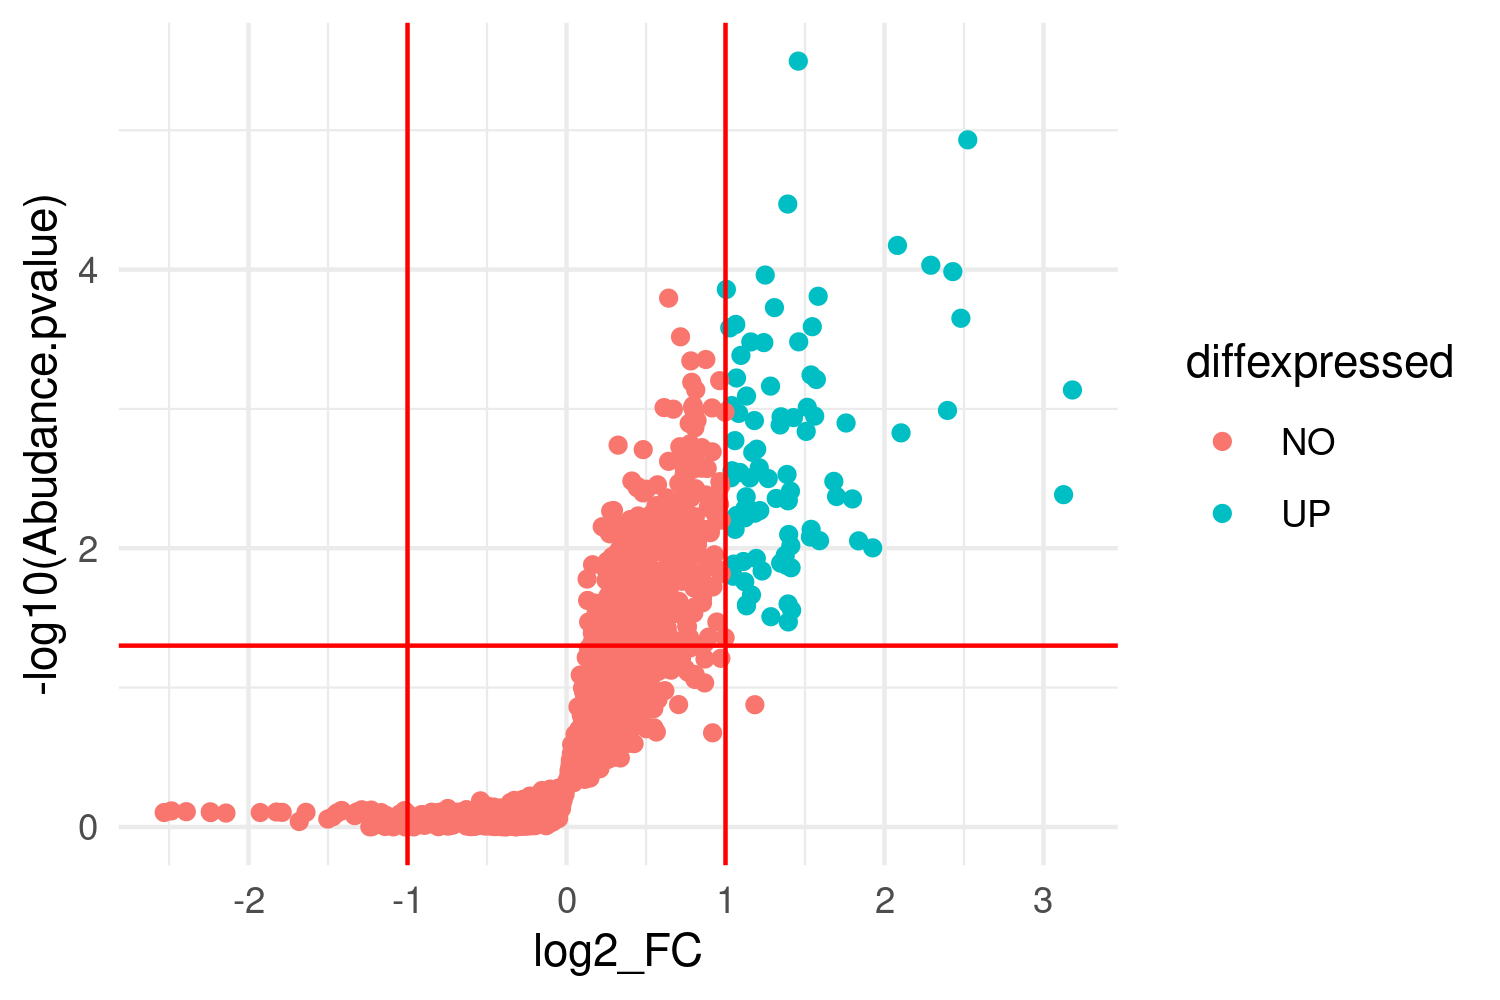
\includegraphics{images/Zoomed_out_Volcano.png}
\caption{Overwiev Volcano Phosho}
\end{figure}

\begin{figure}
\centering
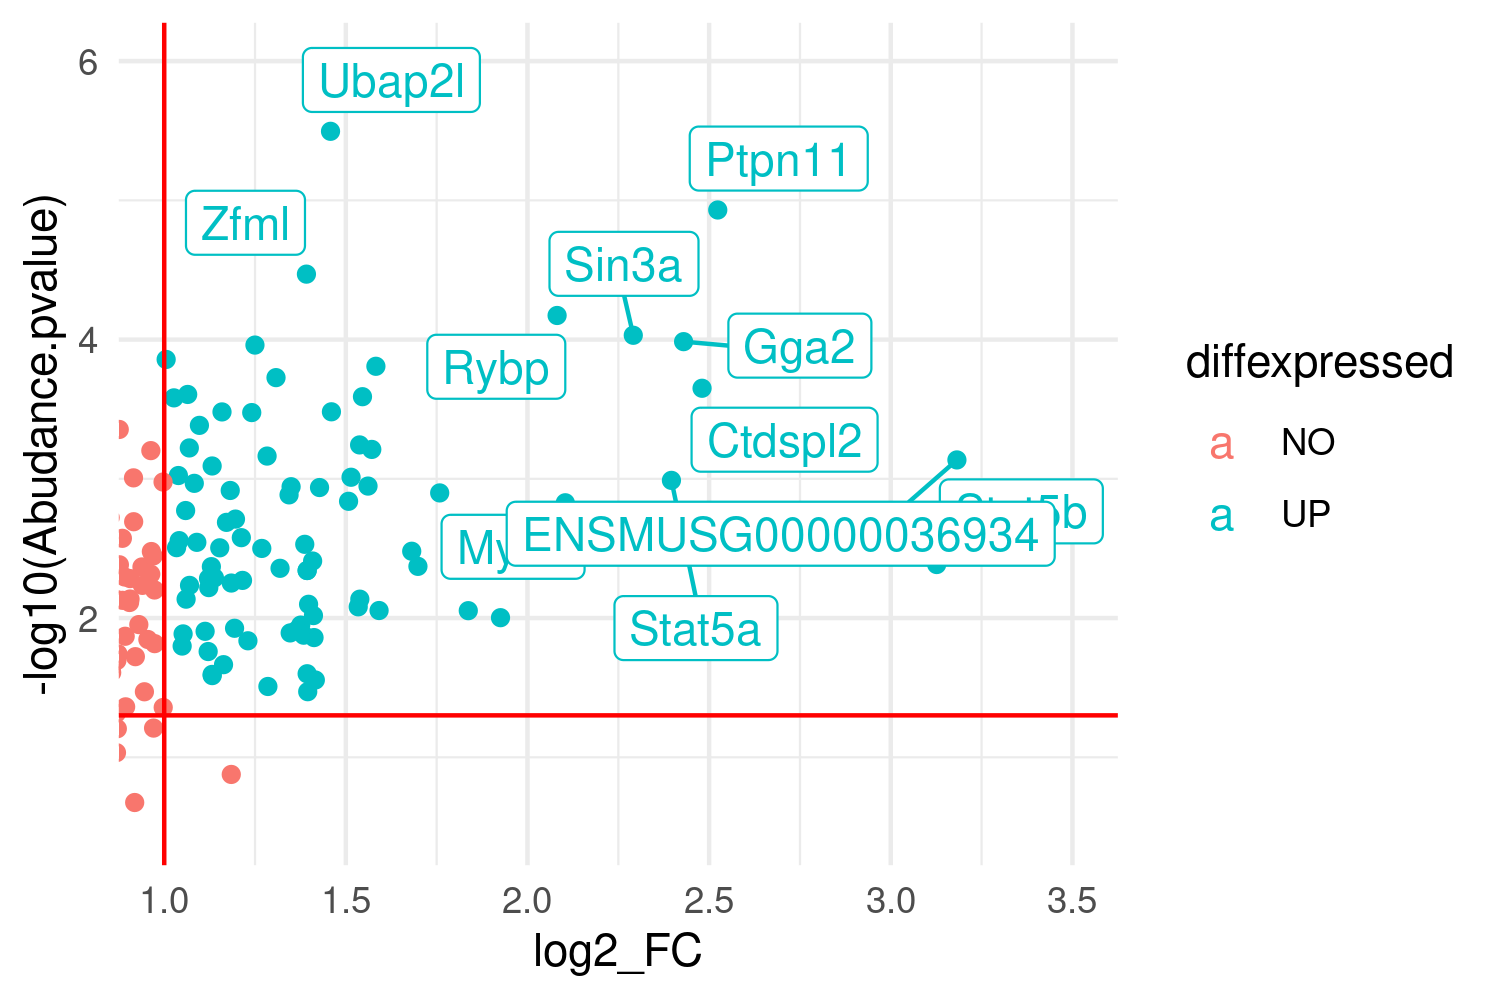
\includegraphics{images/Zoomed_in_Volcano.png}
\caption{Zoomed in Volcano plot Phospho}
\end{figure}

\begin{center}\rule{0.5\linewidth}{0.5pt}\end{center}

\hypertarget{proteome-volcano-plot}{%
\paragraph{Proteome volcano plot}\label{proteome-volcano-plot}}

\begin{itemize}
\tightlist
\item
  Also plotting the proteome data to identify thresholds to clean data
\end{itemize}

\begin{Shaded}
\begin{Highlighting}[]
\CommentTok{\# Defining function first}
\NormalTok{volcano\_plot\_proteome }\OtherTok{\textless{}{-}} \ControlFlowTok{function}\NormalTok{(proteome)\{}
\NormalTok{proteome}\SpecialCharTok{$}\NormalTok{log2\_FC }\OtherTok{\textless{}{-}} \FunctionTok{log2}\NormalTok{(proteome}\SpecialCharTok{$}\NormalTok{Abundance.Ratio...LIF.....Control.)}
\NormalTok{proteome}\SpecialCharTok{$}\NormalTok{diffexpressed }\OtherTok{\textless{}{-}} \StringTok{"NO"}
\NormalTok{proteome}\SpecialCharTok{$}\NormalTok{diffexpressed[proteome}\SpecialCharTok{$}\NormalTok{log2\_FC }\SpecialCharTok{\textgreater{}} \DecValTok{1} \SpecialCharTok{\&}\NormalTok{ proteome}\SpecialCharTok{$}\NormalTok{Abundance.Ratio.P.Value...LIF.....Control. }\SpecialCharTok{\textless{}} \FloatTok{0.05}\NormalTok{] }\OtherTok{\textless{}{-}} \StringTok{"UP"}
\NormalTok{proteome}\SpecialCharTok{$}\NormalTok{diffexpressed[proteome}\SpecialCharTok{$}\NormalTok{log2\_FC }\SpecialCharTok{\textless{}} \SpecialCharTok{{-}}\DecValTok{1} \SpecialCharTok{\&}\NormalTok{ proteome}\SpecialCharTok{$}\NormalTok{Abundance.Ratio.P.Value...LIF.....Control. }\SpecialCharTok{\textless{}} \FloatTok{0.05}\NormalTok{] }\OtherTok{\textless{}{-}} \StringTok{"DOWN"}

\FunctionTok{ggplot}\NormalTok{(}\AttributeTok{data=}\NormalTok{proteome, }\FunctionTok{aes}\NormalTok{(}\AttributeTok{x=}\NormalTok{log2\_FC, }\AttributeTok{y=}\SpecialCharTok{{-}}\FunctionTok{log10}\NormalTok{(Abundance.Ratio.P.Value...LIF.....Control.), }\AttributeTok{col=}\NormalTok{diffexpressed))}\SpecialCharTok{+}
  \FunctionTok{geom\_point}\NormalTok{()}\SpecialCharTok{+}
  \FunctionTok{theme\_minimal}\NormalTok{()}\SpecialCharTok{+}
  \FunctionTok{geom\_vline}\NormalTok{(}\AttributeTok{xintercept=}\FunctionTok{c}\NormalTok{(}\SpecialCharTok{{-}}\DecValTok{1}\NormalTok{, }\DecValTok{1}\NormalTok{), }\AttributeTok{col=}\StringTok{"red"}\NormalTok{) }\SpecialCharTok{+}
  \FunctionTok{geom\_hline}\NormalTok{(}\AttributeTok{yintercept=}\SpecialCharTok{{-}}\FunctionTok{log10}\NormalTok{(}\FloatTok{0.05}\NormalTok{), }\AttributeTok{col=}\StringTok{"red"}\NormalTok{)}
\NormalTok{\}}
\CommentTok{\#Printing the volcano plot}
\FunctionTok{volcano\_plot\_proteome}\NormalTok{(raw\_data\_proteom) }\CommentTok{\# Plots all the data }
\end{Highlighting}
\end{Shaded}

\begin{verbatim}
## Warning: Removed 852 rows containing missing values (geom_point).
\end{verbatim}

\includegraphics{Phosphoproteomics_code_files/figure-latex/unnamed-chunk-8-1.pdf}

\begin{itemize}
\tightlist
\item
  No values are significantly up or down regulated (defining up / down
  regulated as at least 2-fold increase/decrease). Also outliers could
  be observed (4 vales with a \textgreater2-fold increase with
  non-significant p-values). To be more restrictive and decrease the
  change of false positives in the upcoming analysis, also significantly
  increased values with a ratio \textgreater{} 1 were selected as
  undesired data and are going to be removed in the following cleaning
  steps.
\end{itemize}

\begin{center}\rule{0.5\linewidth}{0.5pt}\end{center}

\hypertarget{subsetting-data_phospho-for-ratio-values-2-and-p-values-0.05}{%
\paragraph{Subsetting data\_phospho for ratio values \textgreater= 2 and
p-values \textless=
0.05}\label{subsetting-data_phospho-for-ratio-values-2-and-p-values-0.05}}

\begin{itemize}
\item
  \begin{enumerate}
  \def\labelenumi{\alph{enumi}.}
  \tightlist
  \item
    Remove peptides without quantitative values -\textgreater{} Already
    done in ``If loop to omit na.value from all Abundance columns''
    thereby creating the data\_phospho
  \end{enumerate}
\item
  Here we use the identified thresholds from the volcano plots to clean
  the data. First we select rows with ratio \textgreater= 2 and p.values
  \textless= 0.05 from the phopho dataset. From the proteom data set
  values were selected with a all rows with a ratio \textless= 1, all
  rows with a ratio \textgreater= 1 \textgreater= 2 and p.value
  \textgreater= 0.05 (significant p-values are excluded and ratios
  \textgreater{} bigger than 2 too). After this initial cleanup a
  semi\_join() was performed return all rows from cleanup phospho with a
  match in cleanup proteome, to select only phospo values that showed
  increased phosphorylation due to the LIF treatment.
\item
  volcano plots were used to visualize the cleaning/selecting steps
\end{itemize}

\begin{Shaded}
\begin{Highlighting}[]
\DocumentationTok{\#\#Filter NA out in proteome, Filter out p.values that are non significant(not adjusted)}
  \CommentTok{\#securing no overwrite to original data}
\NormalTok{df\_phospho }\OtherTok{=}\NormalTok{ data\_phospho}
\NormalTok{df\_proteome }\OtherTok{=}\NormalTok{ raw\_data\_proteom}
  
\DocumentationTok{\#\# Filter PHOSPHO}
\NormalTok{  more\_phospho }\OtherTok{\textless{}{-}} \FunctionTok{subset.data.frame}\NormalTok{(df\_phospho, }\AttributeTok{subset =}\NormalTok{ df\_phospho}\SpecialCharTok{$}\NormalTok{Abudance.Ratio }\SpecialCharTok{\textgreater{}=} \DecValTok{2}\NormalTok{) }\CommentTok{\#Filters out all ratios below 2{-}fold}
\NormalTok{  more\_phospho }\OtherTok{\textless{}{-}} \FunctionTok{subset.data.frame}\NormalTok{(more\_phospho, }\AttributeTok{subset =}\NormalTok{ more\_phospho}\SpecialCharTok{$}\NormalTok{Abudance.pvalue }\SpecialCharTok{\textless{}=} \FloatTok{0.05}\NormalTok{) }\CommentTok{\#Filters out all non{-}significant p{-}values}
  
  \DocumentationTok{\#\#Filter PROTEOME}
\NormalTok{  exclude\_proteome }\OtherTok{\textless{}{-}} \FunctionTok{filter}\NormalTok{(df\_proteome, df\_proteome}\SpecialCharTok{$}\NormalTok{Abundance.Ratio.P.Value...LIF.....Control. }\SpecialCharTok{\textless{}=} \FloatTok{0.05} \SpecialCharTok{\&}\NormalTok{ df\_proteome}\SpecialCharTok{$}\NormalTok{Abundance.Ratio...LIF.....Control. }\SpecialCharTok{\textgreater{}=} \DecValTok{1}\NormalTok{) }\CommentTok{\#Filters out all significant p{-}values, because significant p{-}values indicate an }
  \CommentTok{\#Data that we want to exclude, testing if the right data is selected with the volcano plot}
  \FunctionTok{volcano\_plot\_proteome}\NormalTok{(exclude\_proteome)}
\end{Highlighting}
\end{Shaded}

\includegraphics{Phosphoproteomics_code_files/figure-latex/unnamed-chunk-9-1.pdf}

\begin{Shaded}
\begin{Highlighting}[]
  \CommentTok{\#Anti\_join anti\_join() return all rows from x without a match in y. }
\NormalTok{  more\_proteome }\OtherTok{\textless{}{-}} \FunctionTok{anti\_join}\NormalTok{(df\_proteome, exclude\_proteome, }\AttributeTok{by =} \FunctionTok{c}\NormalTok{(}\StringTok{"Accession"} \OtherTok{=} \StringTok{"Accession"}\NormalTok{))}
\NormalTok{  more\_proteome }\OtherTok{\textless{}{-}} \FunctionTok{filter}\NormalTok{(more\_proteome, more\_proteome}\SpecialCharTok{$}\NormalTok{Abundance.Ratio...LIF.....Control. }\SpecialCharTok{\textless{}=} \DecValTok{2}\NormalTok{) }\CommentTok{\# removes outliers with ratio bigger then 2}
  \CommentTok{\#Checking the if the right data is excluded}
  \FunctionTok{volcano\_plot\_proteome}\NormalTok{(more\_proteome)}
\end{Highlighting}
\end{Shaded}

\includegraphics{Phosphoproteomics_code_files/figure-latex/unnamed-chunk-9-2.pdf}

\begin{Shaded}
\begin{Highlighting}[]
  \CommentTok{\#Inner join works too, but semi join is better becasue the proteome columns are not included into the resulting data frame.}
  \CommentTok{\#more\_phosphorylated \textless{}{-} dplyr::inner\_join( more\_phospho, more\_proteome, by = c("Master.Protein.Accessions" = "Accession"))}
  
  \CommentTok{\#Semi{-}join \#semi\_join() return all rows from x with a match in y. }
\NormalTok{  more\_phosphorylated }\OtherTok{\textless{}{-}}\NormalTok{ dplyr}\SpecialCharTok{::}\FunctionTok{semi\_join}\NormalTok{(more\_phospho, more\_proteome, }\AttributeTok{by =} \FunctionTok{c}\NormalTok{(}\StringTok{"Master.Protein.Accessions"} \OtherTok{=} \StringTok{"Accession"}\NormalTok{))}
  \FunctionTok{volcano\_phospho\_plot}\NormalTok{(more\_phosphorylated, }\DecValTok{2}\NormalTok{) }\CommentTok{\# to control remaining data}
  
\FunctionTok{remove}\NormalTok{(df\_phospho, df\_proteome, more\_phospho, more\_proteome, exclude\_proteome)}
\end{Highlighting}
\end{Shaded}

\begin{center}\rule{0.5\linewidth}{0.5pt}\end{center}

\hypertarget{comparing-data-before-and-after-the-cleanup}{%
\paragraph{Comparing data before and after the
cleanup}\label{comparing-data-before-and-after-the-cleanup}}

-we could identify that the cleanup was conducted and not too stringent
returning enough data to conduct analyisis on.

\begin{center}\rule{0.5\linewidth}{0.5pt}\end{center}

\hypertarget{volcano-of-data_phospho-before-filterzoomed-in-volcano-from-more-phosphorylated-after-filter}{%
\paragraph{\texorpdfstring{\protect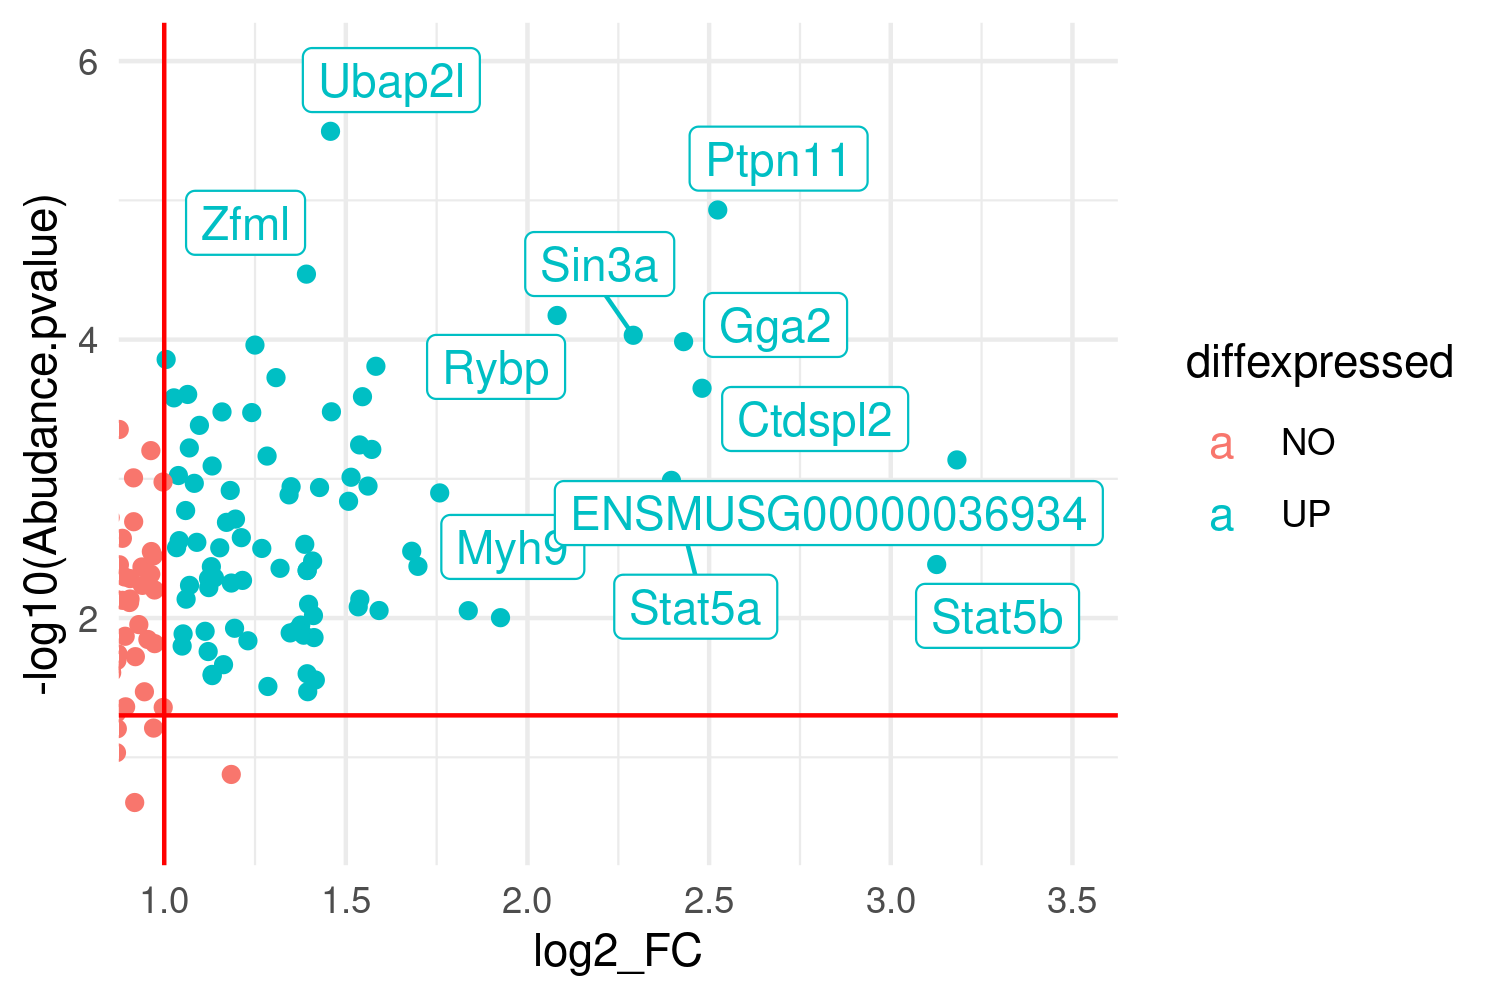
\includegraphics[width=3.64583in,height=\textheight]{images/Zoomed_in_Volcano-01.png}\protect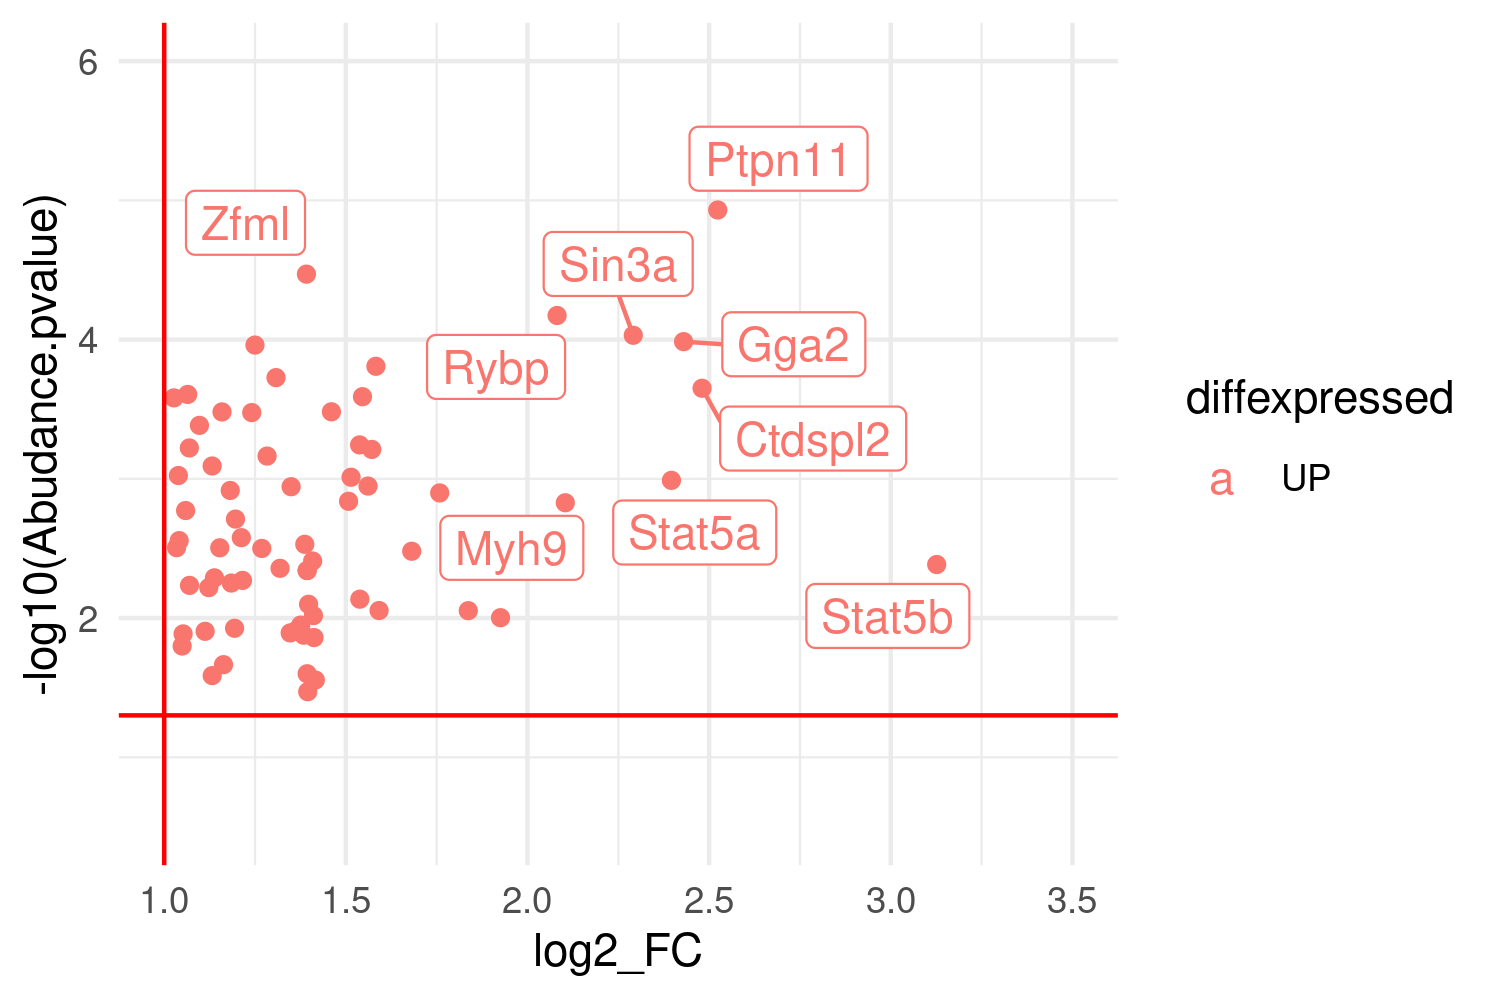
\includegraphics[width=3.64583in,height=\textheight]{images/Zoomed_in_Volcano_for_more_phosphrylated_after_qc_and_filter.png}}{Volcano of data\_phospho before filterZoomed in Volcano from more phosphorylated after filter}}\label{volcano-of-data_phospho-before-filterzoomed-in-volcano-from-more-phosphorylated-after-filter}}

\begin{center}\rule{0.5\linewidth}{0.5pt}\end{center}

\hypertarget{section}{%
\paragraph{}\label{section}}

\hypertarget{building-network-map-of-the-proteins}{%
\paragraph{Building network map of the
proteins}\label{building-network-map-of-the-proteins}}

\begin{itemize}
\tightlist
\item
  With help of the STRINgdb package the overview networks were produced
  with different thresholds.
\end{itemize}

\begin{Shaded}
\begin{Highlighting}[]
\DocumentationTok{\#\#Lower score\_threshold, allowing more connections}
\NormalTok{string\_db\_low }\OtherTok{\textless{}{-}}\NormalTok{ STRINGdb}\SpecialCharTok{$}\FunctionTok{new}\NormalTok{(}\AttributeTok{version=}\StringTok{"11.5"}\NormalTok{, }\AttributeTok{species=}\DecValTok{10090}\NormalTok{, }\AttributeTok{score\_threshold=}\DecValTok{1}\NormalTok{, }\AttributeTok{input\_directory=}\StringTok{""}\NormalTok{) }\CommentTok{\#species = mouse identifier, score threshold = if one interaction this will be mapped, no input directory data stored only temporary}
\NormalTok{hits\_low }\OtherTok{\textless{}{-}}\NormalTok{ string\_db\_low}\SpecialCharTok{$}\FunctionTok{map}\NormalTok{(more\_phosphorylated, }\StringTok{"Master.Protein.Accessions"}\NormalTok{, }\AttributeTok{removeUnmappedRows =}\NormalTok{ F) }\CommentTok{\#mapping the UNIPROT Ids from the first column to get STRING identifiers}

\NormalTok{string\_db\_low}\SpecialCharTok{$}\FunctionTok{plot\_network}\NormalTok{(hits\_low}\SpecialCharTok{$}\NormalTok{STRING\_id) }\CommentTok{\#plotting network}
\end{Highlighting}
\end{Shaded}

\includegraphics{Phosphoproteomics_code_files/figure-latex/unnamed-chunk-10-1.pdf}

\begin{Shaded}
\begin{Highlighting}[]
\FunctionTok{invisible}\NormalTok{(string\_db\_low}\SpecialCharTok{$}\FunctionTok{get\_png}\NormalTok{(hits\_low}\SpecialCharTok{$}\NormalTok{STRING\_id, }\AttributeTok{file =} \StringTok{"\textasciitilde{}/phosphoproteomics\_project/results/Network\_low.png"}\NormalTok{)) }\CommentTok{\#Saving photo}

\DocumentationTok{\#\# Higher score\_threshold, allowing less connections}
\NormalTok{string\_db\_high }\OtherTok{\textless{}{-}}\NormalTok{ STRINGdb}\SpecialCharTok{$}\FunctionTok{new}\NormalTok{(}\AttributeTok{version=}\StringTok{"11.5"}\NormalTok{, }\AttributeTok{species=}\DecValTok{10090}\NormalTok{, }\AttributeTok{score\_threshold=}\DecValTok{200}\NormalTok{, }\AttributeTok{input\_directory=}\StringTok{""}\NormalTok{) }\CommentTok{\#species = mouse identifier, score threshold = if one interaction this will be mapped, no input directory data stored only temporary}
\NormalTok{hits\_high }\OtherTok{\textless{}{-}}\NormalTok{ string\_db\_high}\SpecialCharTok{$}\FunctionTok{map}\NormalTok{(more\_phosphorylated, }\StringTok{"Master.Protein.Accessions"}\NormalTok{, }\AttributeTok{removeUnmappedRows =}\NormalTok{ F) }\CommentTok{\#mapping the UNIPROT Ids from the first column to get STRING identifiers}

\NormalTok{string\_db\_high}\SpecialCharTok{$}\FunctionTok{plot\_network}\NormalTok{(hits\_high}\SpecialCharTok{$}\NormalTok{STRING\_id) }\CommentTok{\#plotting network}
\end{Highlighting}
\end{Shaded}

\includegraphics{Phosphoproteomics_code_files/figure-latex/unnamed-chunk-10-2.pdf}

\begin{Shaded}
\begin{Highlighting}[]
\FunctionTok{invisible}\NormalTok{(string\_db\_high}\SpecialCharTok{$}\FunctionTok{get\_png}\NormalTok{(hits\_high}\SpecialCharTok{$}\NormalTok{STRING\_id, }\AttributeTok{file =} \StringTok{"\textasciitilde{}/phosphoproteomics\_project/results/Network\_high.png"}\NormalTok{)) }\CommentTok{\#Saving photo}
\end{Highlighting}
\end{Shaded}

\begin{center}\rule{0.5\linewidth}{0.5pt}\end{center}

\hypertarget{way-to-identify-the-proteins-stat5b-is-connected-to.}{%
\paragraph{Way to identify the Proteins Stat5b is connected
to.}\label{way-to-identify-the-proteins-stat5b-is-connected-to.}}

\begin{itemize}
\item
  In this chunk we define a function with a more and a less stringent
  threshold to get 1. Proteins\_connected\_to\_Stat5b for more or less
  stringent threshold, 2. Network plot for the subnetworks of proteins
  connected to Stat5b, 3. Link to webpage for the subnetworks, 4.
  Pathways that are enriched in the subnetworks.
\item
  There is also a link to the
  \href{https://version-11-5.string-db.org/cgi/link?to=2E8CDC990DBD10F7}{STRINGdb
  website for less stringent threshold = 1} with the Proteins connected
  to Stat5b in this dataset.
\item
  There is also a link to the
  \href{https://version-11-5.string-db.org/cgi/link?to=18B5C3E16E9B3AE0}{STRINGdb
  website for more stringent threshold = 200} with the Proteins
  connected to Stat5b in this dataset.
\end{itemize}

\begin{Shaded}
\begin{Highlighting}[]
\CommentTok{\#Finding String id identifier for Stat5b and assigning it to the a variable}
\NormalTok{i }\OtherTok{\textless{}{-}} \FunctionTok{grep}\NormalTok{(}\StringTok{"P42232"}\NormalTok{, hits\_low}\SpecialCharTok{$}\NormalTok{Master.Protein.Accessions) }
\NormalTok{Stat5b }\OtherTok{\textless{}{-}}\NormalTok{ string\_db\_low}\SpecialCharTok{$}\FunctionTok{mp}\NormalTok{(}\StringTok{"P42232"}\NormalTok{) }\CommentTok{\#mapping the UNIPROT Ids }

\DocumentationTok{\#\# Mapping Stat5b interactions in the less stringent data set and more stringent data set}

\CommentTok{\#Defining a function to get 1. Proteins\_connected\_to\_Stat5b, 2. Network plot, 3. Link to webpage, 4. Pathways}
\NormalTok{subnetworks }\OtherTok{\textless{}{-}} \ControlFlowTok{function}\NormalTok{(data\_h,score\_h) \{}
  \CommentTok{\#a = The data we want to have a network from, b = the threshold number of the string\_db function}
\NormalTok{  string\_db }\OtherTok{\textless{}{-}}\NormalTok{ STRINGdb}\SpecialCharTok{$}\FunctionTok{new}\NormalTok{(}\AttributeTok{version=}\StringTok{"11.5"}\NormalTok{, }\AttributeTok{species=}\DecValTok{10090}\NormalTok{, }\AttributeTok{score\_threshold =}\NormalTok{ score\_h, }\AttributeTok{input\_directory=}\StringTok{""}\NormalTok{) }\CommentTok{\#species = mouse }
\NormalTok{  get }\OtherTok{\textless{}{-}}\NormalTok{ string\_db}\SpecialCharTok{$}\FunctionTok{get\_subnetwork}\NormalTok{(data\_h) }\CommentTok{\#builds subnetwork from every entry in STRING\_id}
\NormalTok{  ghi }\OtherTok{\textless{}{-}}\NormalTok{ get[[Stat5b]][}\DecValTok{1}\NormalTok{] }\DocumentationTok{\#\#gives the list entry of "get" that lists all 18 entries that interact with Stat5b}
\NormalTok{  hg }\OtherTok{\textless{}{-}} \FunctionTok{unique}\NormalTok{(ghi}\SpecialCharTok{$}\StringTok{\textasciigrave{}}\AttributeTok{10090.ENSMUSP00000102981}\StringTok{\textasciigrave{}}\NormalTok{) }\CommentTok{\#gives the unique interaction (9 out of 18), }
\NormalTok{  mat }\OtherTok{\textless{}{-}} \FunctionTok{as\_ids}\NormalTok{(ghi}\SpecialCharTok{$}\StringTok{\textasciigrave{}}\AttributeTok{10090.ENSMUSP00000102981}\StringTok{\textasciigrave{}}\NormalTok{) }\CommentTok{\#function as\_ids from the igraph package reads the class("igraph.vs")   and collapses it into a matrix}
\NormalTok{  Proteins\_connected\_to\_Stat5b }\OtherTok{\textless{}{-}} \FunctionTok{as.data.frame}\NormalTok{(}\FunctionTok{unique}\NormalTok{(mat))}
  \FunctionTok{names}\NormalTok{(Proteins\_connected\_to\_Stat5b)[}\DecValTok{1}\NormalTok{] }\OtherTok{\textless{}{-}} \StringTok{"STRING\_id"} \CommentTok{\#Renaming column so that add\_protein\_description recognizes it}
\NormalTok{  Proteins\_connected\_to\_Stat5b[(}\FunctionTok{nrow}\NormalTok{(Proteins\_connected\_to\_Stat5b)}\SpecialCharTok{+}\DecValTok{1}\NormalTok{),] }\OtherTok{\textless{}{-}}\NormalTok{ Stat5b }\CommentTok{\#Adds Stat5b to map its connections}
\NormalTok{  Proteins\_connected\_to\_Stat5b }\OtherTok{\textless{}{-}}\NormalTok{ string\_db}\SpecialCharTok{$}\FunctionTok{add\_proteins\_description}\NormalTok{(Proteins\_connected\_to\_Stat5b) }\CommentTok{\#Add´s protein information to STRINGid´s}
  
  \CommentTok{\#Plotting the subnetwork}
\NormalTok{  string\_db}\SpecialCharTok{$}\FunctionTok{plot\_network}\NormalTok{(Proteins\_connected\_to\_Stat5b}\SpecialCharTok{$}\NormalTok{STRING\_id)}
  
  \CommentTok{\#providing my link}
\NormalTok{  link }\OtherTok{\textless{}{-}}\NormalTok{ string\_db}\SpecialCharTok{$}\FunctionTok{get\_link}\NormalTok{(Proteins\_connected\_to\_Stat5b}\SpecialCharTok{$}\NormalTok{STRING\_id) }\CommentTok{\#Provides link to the STRINGdb page}
  
  \CommentTok{\#Providing the pathways}
\NormalTok{  pathways }\OtherTok{\textless{}{-}}\NormalTok{ string\_db}\SpecialCharTok{$}\FunctionTok{get\_enrichment}\NormalTok{(Proteins\_connected\_to\_Stat5b, }\AttributeTok{category =} \StringTok{"KEGG"}\NormalTok{)}

  \FunctionTok{return}\NormalTok{(}\FunctionTok{list}\NormalTok{(Proteins\_connected\_to\_Stat5b, pathways, link))}
  
  \FunctionTok{remove}\NormalTok{(get,ghi,hg,mat)}
\NormalTok{   \}}

\DocumentationTok{\#\# Less stringent parameter to determine the Proteins that interact with Stat5}
\NormalTok{subnetwork\_less\_stringent }\OtherTok{\textless{}{-}} \FunctionTok{subnetworks}\NormalTok{(}\AttributeTok{data\_h =}\NormalTok{ hits\_low}\SpecialCharTok{$}\NormalTok{STRING\_id, }\AttributeTok{score\_h =} \DecValTok{1}\NormalTok{) }\CommentTok{\#Using function}
\end{Highlighting}
\end{Shaded}

\includegraphics{Phosphoproteomics_code_files/figure-latex/unnamed-chunk-11-1.pdf}

\begin{Shaded}
\begin{Highlighting}[]
\CommentTok{\#Sub{-}setting the returned list into original dataframes + link}
\NormalTok{Proteins\_connected\_to\_Stat5b\_less }\OtherTok{\textless{}{-}}\NormalTok{ subnetwork\_less\_stringent[[}\DecValTok{1}\NormalTok{]]}
\NormalTok{pathways\_less }\OtherTok{\textless{}{-}}\NormalTok{ subnetwork\_less\_stringent[[}\DecValTok{2}\NormalTok{]]}
\NormalTok{Link\_less }\OtherTok{\textless{}{-}}\NormalTok{ subnetwork\_less\_stringent[[}\DecValTok{3}\NormalTok{]]}
\NormalTok{Link\_less }\CommentTok{\#Link to website}
\end{Highlighting}
\end{Shaded}

\begin{verbatim}
## [1] "https://version-11-5.string-db.org/cgi/link?to=2E8CDC990DBD10F7"
\end{verbatim}

\begin{Shaded}
\begin{Highlighting}[]
\FunctionTok{invisible}\NormalTok{(string\_db\_low}\SpecialCharTok{$}\FunctionTok{get\_png}\NormalTok{(Proteins\_connected\_to\_Stat5b\_less}\SpecialCharTok{$}\NormalTok{STRING\_id, }\AttributeTok{file =} \StringTok{"\textasciitilde{}/phosphoproteomics\_project/results/Network\_Stat5\_less.png"}\NormalTok{)) }\CommentTok{\#Saving png}

\DocumentationTok{\#\# More stringent parameter to determine the Proteins that interact with Stat5}
\NormalTok{subnetwork\_more\_stringent }\OtherTok{\textless{}{-}} \FunctionTok{subnetworks}\NormalTok{(}\AttributeTok{data\_h =}\NormalTok{ hits\_high}\SpecialCharTok{$}\NormalTok{STRING\_id, }\AttributeTok{score\_h =} \DecValTok{200}\NormalTok{) }\CommentTok{\#Using function}
\end{Highlighting}
\end{Shaded}

\includegraphics{Phosphoproteomics_code_files/figure-latex/unnamed-chunk-11-2.pdf}

\begin{Shaded}
\begin{Highlighting}[]
\CommentTok{\#Sub{-}setting the returned list into original dataframes + link}
\NormalTok{Proteins\_connected\_to\_Stat5b\_more }\OtherTok{\textless{}{-}}\NormalTok{ subnetwork\_more\_stringent[[}\DecValTok{1}\NormalTok{]] }
\NormalTok{pathways\_more }\OtherTok{\textless{}{-}}\NormalTok{ subnetwork\_more\_stringent[[}\DecValTok{2}\NormalTok{]]}
\NormalTok{Link\_more }\OtherTok{\textless{}{-}}\NormalTok{ subnetwork\_more\_stringent[[}\DecValTok{3}\NormalTok{]]}
\NormalTok{Link\_more }\CommentTok{\#Link to website }
\end{Highlighting}
\end{Shaded}

\begin{verbatim}
## [1] "https://version-11-5.string-db.org/cgi/link?to=18B5C3E16E9B3AE0"
\end{verbatim}

\begin{Shaded}
\begin{Highlighting}[]
\FunctionTok{invisible}\NormalTok{(string\_db\_high}\SpecialCharTok{$}\FunctionTok{get\_png}\NormalTok{(Proteins\_connected\_to\_Stat5b\_more}\SpecialCharTok{$}\NormalTok{STRING\_id, }\AttributeTok{file =} \StringTok{"\textasciitilde{}/phosphoproteomics\_project/results/Network\_Stat5\_more.png"}\NormalTok{)) }\CommentTok{\#Saving png}
\end{Highlighting}
\end{Shaded}

\begin{center}\rule{0.5\linewidth}{0.5pt}\end{center}

\hypertarget{printing-pathways}{%
\paragraph{Printing Pathways}\label{printing-pathways}}

-printing the enriched pathways from the subnetworks of Stat5b and
renaming them for a better human readability \& formatting of html
document.

\begin{Shaded}
\begin{Highlighting}[]
\CommentTok{\#Identifying only for Proteins connected to Stat5b}

\CommentTok{\#Function to generate tabels based on factor gene counts / number of annotated genes.}
\NormalTok{factor\_function }\OtherTok{\textless{}{-}} \ControlFlowTok{function}\NormalTok{(Pathway)\{}
\NormalTok{i }\OtherTok{=} \DecValTok{1}
\ControlFlowTok{for}\NormalTok{ (i }\ControlFlowTok{in}\NormalTok{ i}\SpecialCharTok{:}\FunctionTok{nrow}\NormalTok{(Pathway)) \{}
\NormalTok{  Pathway}\SpecialCharTok{$}\NormalTok{factor[i] }\OtherTok{\textless{}{-}} \FunctionTok{round}\NormalTok{((Pathway[i,}\DecValTok{3}\NormalTok{]}\SpecialCharTok{/}\NormalTok{Pathway[i,}\DecValTok{4}\NormalTok{]), }\AttributeTok{digits =} \DecValTok{3}\NormalTok{) }\CommentTok{\#rounded for better visualization}
\NormalTok{\}}
\NormalTok{Pathway }\OtherTok{\textless{}{-}} \FunctionTok{rename}\NormalTok{(Pathway, }\AttributeTok{background =}\NormalTok{ number\_of\_genes\_in\_background)}
\NormalTok{Pathway }\OtherTok{\textless{}{-}} \FunctionTok{rename}\NormalTok{(Pathway, }\AttributeTok{hits =}\NormalTok{ number\_of\_genes)}
\NormalTok{Pathway }\OtherTok{\textless{}{-}} \FunctionTok{rename}\NormalTok{(Pathway, }\AttributeTok{involved\_genes =}\NormalTok{ preferredNames)}
\NormalTok{Pathway }\OtherTok{\textless{}{-}}\NormalTok{ Pathway[}\FunctionTok{order}\NormalTok{(Pathway}\SpecialCharTok{$}\NormalTok{factor,}\AttributeTok{decreasing =}\NormalTok{ T ),]}
\FunctionTok{return}\NormalTok{(}\FunctionTok{print.data.frame}\NormalTok{(Pathway[}\DecValTok{1}\SpecialCharTok{:}\DecValTok{5}\NormalTok{,}\FunctionTok{c}\NormalTok{(}\DecValTok{11}\NormalTok{,}\DecValTok{3}\NormalTok{,}\DecValTok{4}\NormalTok{,}\DecValTok{10}\NormalTok{,}\DecValTok{7}\NormalTok{)], }\AttributeTok{row.names =}\NormalTok{ F))}
\NormalTok{\}}
\CommentTok{\#Table for less stringent parameters}
\FunctionTok{factor\_function}\NormalTok{(pathways\_less)}
\end{Highlighting}
\end{Shaded}

\begin{verbatim}
##  factor hits background                 description            involved_genes
##   0.054    4         74    Chronic myeloid leukemia Stat5a,Sos1,Ptpn11,Stat5b
##   0.045    3         66  Non-small cell lung cancer        Stat5a,Sos1,Stat5b
##   0.043    3         70      Acute myeloid leukemia        Stat5a,Sos1,Stat5b
##   0.041    3         74 Prolactin signaling pathway        Stat5a,Sos1,Stat5b
##   0.037    3         81      ErbB signaling pathway        Stat5a,Sos1,Stat5b
\end{verbatim}

\begin{Shaded}
\begin{Highlighting}[]
\CommentTok{\#Table for more stringent parameters}
\FunctionTok{factor\_function}\NormalTok{(pathways\_more)}
\end{Highlighting}
\end{Shaded}

\begin{verbatim}
##  factor hits background                                          description
##   0.041    3         74                             Chronic myeloid leukemia
##   0.030    3        101 AGE-RAGE signaling pathway in diabetic complications
##   0.018    3        165                           JAK-STAT signaling pathway
##      NA   NA         NA                                                 <NA>
##      NA   NA         NA                                                 <NA>
##        involved_genes
##  Stat5a,Ptpn11,Stat5b
##   Stat5a,Foxo1,Stat5b
##  Stat5a,Ptpn11,Stat5b
##                  <NA>
##                  <NA>
\end{verbatim}

\begin{Shaded}
\begin{Highlighting}[]
\CommentTok{\#Identifying pathways also for Proteins with a ratio \textgreater{}=2 and p.value \textless{}= 0.05 and threshold = 200.}
\NormalTok{Big\_network\_pathways\_more }\OtherTok{\textless{}{-}}\NormalTok{ string\_db\_high}\SpecialCharTok{$}\FunctionTok{get\_enrichment}\NormalTok{(hits\_high}\SpecialCharTok{$}\NormalTok{STRING\_id, }\AttributeTok{category =} \StringTok{"KEGG"}\NormalTok{)}
\FunctionTok{factor\_function}\NormalTok{(Big\_network\_pathways\_more)}
\end{Highlighting}
\end{Shaded}

\begin{verbatim}
##  factor hits background              description            involved_genes
##   0.054    4         74 Chronic myeloid leukemia Stat5a,Sos1,Ptpn11,Stat5b
##   0.049    4         81   ErbB signaling pathway   Stat5a,Gab1,Sos1,Stat5b
##      NA   NA         NA                     <NA>                      <NA>
##      NA   NA         NA                     <NA>                      <NA>
##      NA   NA         NA                     <NA>                      <NA>
\end{verbatim}

\begin{Shaded}
\begin{Highlighting}[]
\CommentTok{\#Identifying pathways also for Proteins with a ratio \textgreater{}=2 and p.value \textless{}= 0.05 and threshold = 1.}
\NormalTok{Big\_network\_pathways\_less }\OtherTok{\textless{}{-}}\NormalTok{ string\_db\_low}\SpecialCharTok{$}\FunctionTok{get\_enrichment}\NormalTok{(hits\_low}\SpecialCharTok{$}\NormalTok{STRING\_id, }\AttributeTok{category =} \StringTok{"KEGG"}\NormalTok{)}
\FunctionTok{factor\_function}\NormalTok{(Big\_network\_pathways\_less)}
\end{Highlighting}
\end{Shaded}

\begin{verbatim}
##  factor hits background              description            involved_genes
##   0.054    4         74 Chronic myeloid leukemia Stat5a,Sos1,Ptpn11,Stat5b
##   0.049    4         81   ErbB signaling pathway   Stat5a,Gab1,Sos1,Stat5b
##      NA   NA         NA                     <NA>                      <NA>
##      NA   NA         NA                     <NA>                      <NA>
##      NA   NA         NA                     <NA>                      <NA>
\end{verbatim}

\begin{Shaded}
\begin{Highlighting}[]
\FunctionTok{remove}\NormalTok{(i, Link\_less, Link\_more, string\_db\_high, string\_db\_low, subnetworks, volcano\_plot\_proteome, subnetwork\_less\_stringent, subnetwork\_more\_stringent, hits\_high, hits\_low, data\_phospho, factor\_function, volcano\_phospho\_plot, string\_db\_volcano)}
\end{Highlighting}
\end{Shaded}

\begin{center}\rule{0.5\linewidth}{0.5pt}\end{center}

\hypertarget{results-and-discussion}{%
\paragraph{Results and Discussion}\label{results-and-discussion}}

\begin{itemize}
\item
  Stat5b was picked as the lead target since it showed the highest
  significant ratio after data clean up in the phospho data set.
\item
  The more stringent parameters turned out less proteins connected to
  Stat5b/5a but with a higher security of true association. The
  generated subnetwork for Stat5b showed a very promising target for
  further investigation, since a real network evolves around Stat5b.
  Generated pathways to investigate the effect of increased
  phosphorylation returned many cancer-related pathways indicating a
  connection between retaining a non-differentiated state in stem cells
  and the capability of cancerous cells to form cancerous masses. Of the
  non-cancer pathways JAK-STAT is of most importance since it's also the
  sub pathway affected in the cancer pathways.
\item
  The less stringent parameters turned out more proteins connected to
  Stat5b/5a but has a higher risk of false positive connections. In the
  follow up pathway analysis this turned out to be irrelevant, since
  major contributions to pathways are done by Stat5b/5a that are part of
  both data sets. This could be seen in the involved\_genes section in
  the data tables. Stat5b forms homo- and hetero dimers especially with
  the paralog Stat5a. Upon Tyr-phosphorylation they dimerize and
  translocate into the nucleus takes place where it acts as
  \href{https://doi.org/10.1074/jbc.274.32.22484}{transcription factor}.
  The more stringent threshold parameter also removed Sos1 from the
  dataset. Sos1 is involved together with Stat5a/b in most of the
  enriched pathways in the less stringent dataset. The Ras-Raf\_MAPK
  pathway is regulated by Sos1, normally acting as guanin nucleotide
  exchange factor \href{https://doi.org/10.1083/jcb.200103146}{upon
  Ras}. Phosphorylation of specific Serin residues have a deactivating
  effect on Sos1 and is used as negative regulator of the
  \href{https://doi.org/10.1042/BJ20120938}{whole Ras-Raf-MAPK pathway},
  a pathway normally associated with
  \href{https://doi.org/10.1002/jcp.28334}{promoting differentiation}.
  Sos1 is also invovled in the mTOR pathway, together with Akt1s1
  (subunit of mTORC1), both also found in the less stringent subnetwork
  but not the more stringent one.

  \begin{figure}
  \centering
  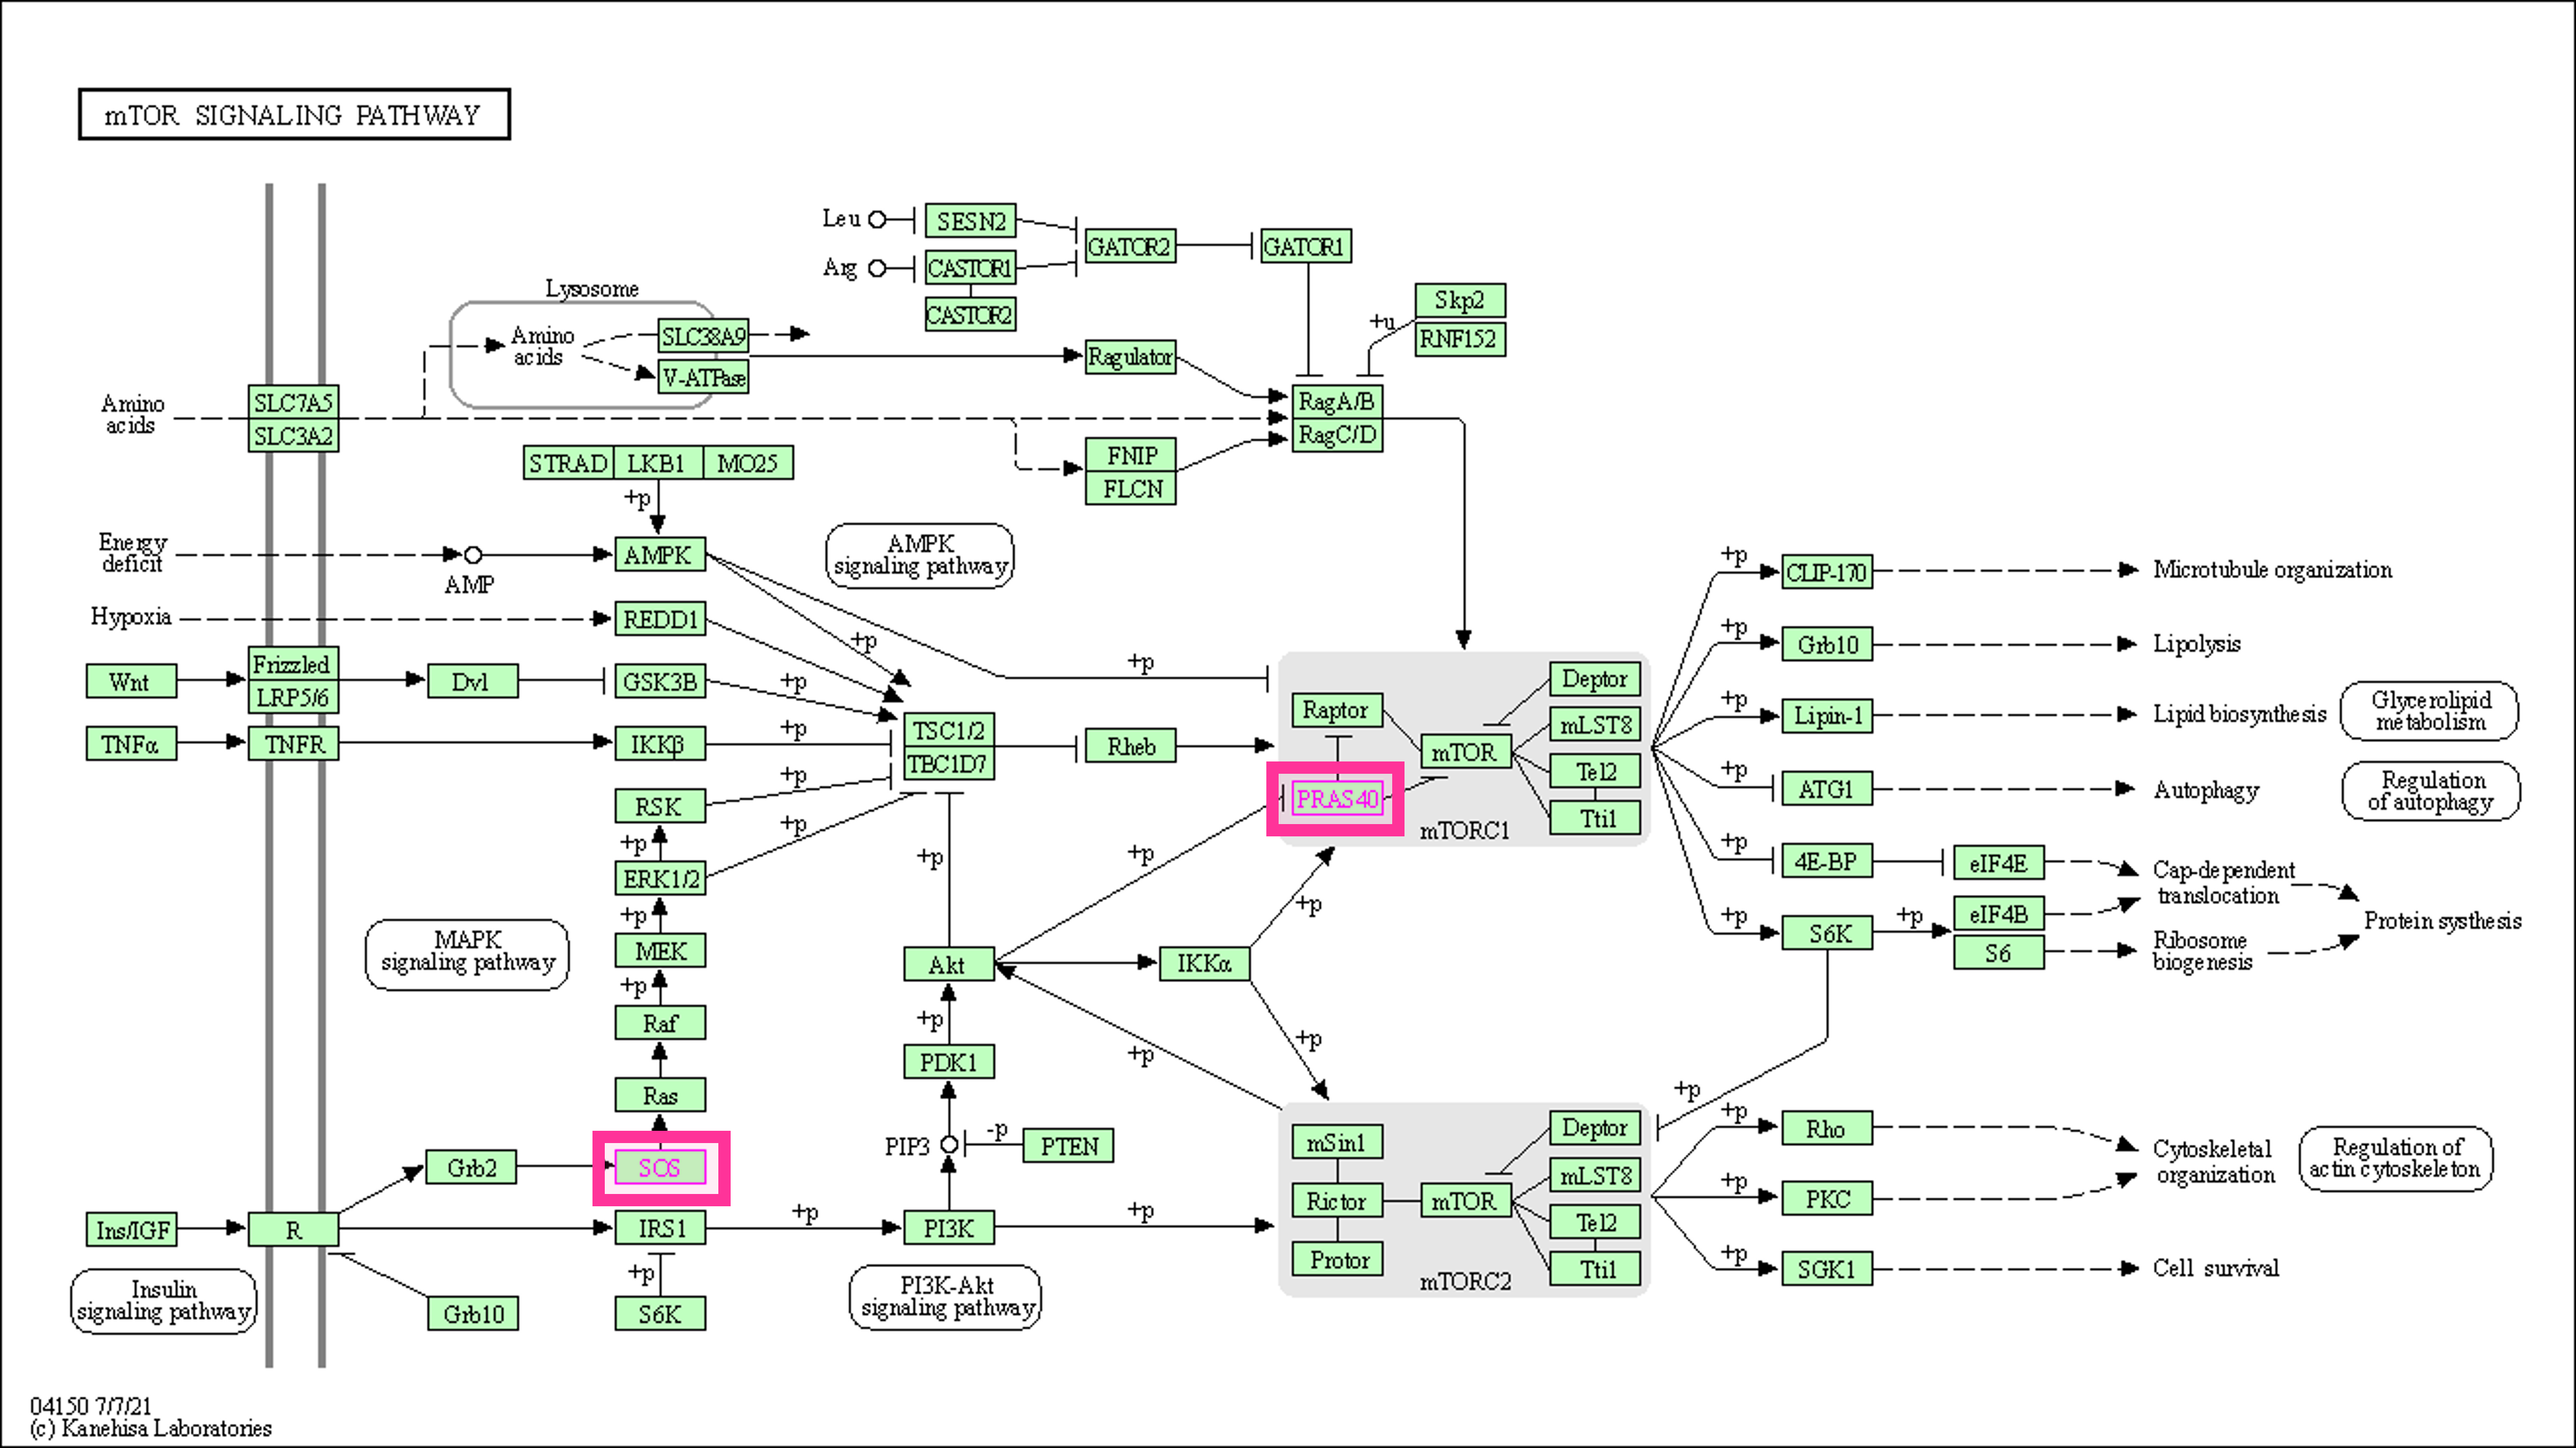
\includegraphics{images/mTOR_pathway.png}
  \caption{mTOR-pathway with Akt1s1 (PRAS40) and Sos1 marked in pink
  from KEGG, entry
  \href{https://www.kegg.jp/pathway/mmu04150}{mmu04150}.}
  \end{figure}
\item
  Under these biological circumstances these founds can be counted as
  valid and are object for further investigation, while other hits in
  the less stringent data set may be found as false positives. This was
  a very good example of the trade-of encountered by threshold settings
  that must be controlled thorough the data analysis.
\end{itemize}

\hypertarget{conclusion}{%
\paragraph{Conclusion}\label{conclusion}}

\begin{itemize}
\tightlist
\item
  Many cancers involved pathways are also activated to ensure stemness
  in non-differentiated muscle mouse cells upon differentiation stimuli.
\item
  Major targets for further investigations are JAK-STAT pathway proteins
  and Sos1 and Akt1s1 with the mTOR- and MAPK-pathway. Especially
  identification of phosphorylation sites in the protein and experiments
  with different differentiation inhibitors to ensure unspecific
  activation of stemness protecting pathways or identification of
  alternatively activated pathways could provide more insights.
\item
  Also, possibly a reproduction of the dataset with more samples to
  identify with a higher security the elevation of involved proteins and
  also reproduction in different cell lines to ensure that the observed
  effects are stemness related and not cell line related would be
  interesting research targets. Since the bioinformatic pipeline is in
  place, the analysis could be conducted quickly.
\end{itemize}

\begin{center}\rule{0.5\linewidth}{0.5pt}\end{center}

\begin{center}\rule{0.5\linewidth}{0.5pt}\end{center}

\end{document}
